\section{Processo de Testes definidos pelo ITRAC}

A busca pela simplificação  e transformação de serviços utilizando das soluções tecnológicas que a empresa terceiriza proporciona está relacionada à problemática de se testar sem requisitos. A transformação digital que se ocorre não garante requisitos estáveis ou, até mesmo, a existência de requisitos e isto pode resultar em um problema definido como Problema do Oráculo~\cite{barr2015oracle}. 

O cenário de requisitos instáveis dificulta a identificação do comportamento atual do serviço digitalizado ao ser comparado com o comportamento esperado, ou ao ser analisado como um comportamento errado.  Além disso, devido a forma de contratação definida, o código-fonte dos serviços transformados não são disponibilizados, o que dificulta mais ainda o processo de testes e a extração de informações por parte da equipe de testes.

Levando todo o contexto da transformação dos serviços em consideração, foi desenvolvido um processo de validação sistematizado, com o intuito de garantira qualidade da digitalização dos serviços. As etapas de criação e execução de casos de teste de cada serviço podem ser realizadas usando diversos padrões de teste, desde estratégias de teste manual até testes automatizados. 

O processo de validação dos serviços digitizados  definido pelo ITRAC está de acordo com o apresentado na Figura \ref{img:process_test}.
 
 \begin{figure}[H]
 \centering
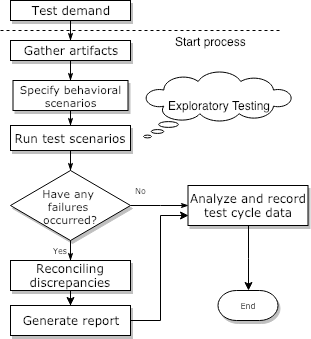
\includegraphics[width=0.7\textwidth]{figuras/Processo_artigo_menor.png}
\caption{Processo de Validação de Serviços definido pelo ITRAC adaptado de~\cite{elcock2006testing}.}
\label{img:process_test}
\end{figure}

Visto que o código-fonte não é acessível pelo ITRAC e o conjunto de requisitos não é bem definido, o processo proposto pelo ITRAC se baseia na estratégia proposta por \cite{elcock2006testing} e no conceito de Teste Exploratório (ET), sugerido por \cite{whittaker2009exploratory}, usando a metáfora do turista como uma estratégia para guiar, através das chamadas ``tours'', a descoberta de requisitos e regras de negócios, além de sistematizar a criação e execução dos casos de teste. O conceito de Testes Exploratórios utilizado como base para definição do processo de teste será apresentado, de maneira detalhada, na Seção \ref{sec:testes_exploratorios}.


A partir da padronização do processo de teste definida pelo ITRAC, foi possível iniciar o desenvolvimento de uma ferramenta de apoio ao processo de teste dos serviços digitizados. A ferramenta, chamada \textit{Digital Transformation Environment Support Tool}, ou DTEST é apresentada a seguir.

\subsection[DTEST]{Ferramenta DTEST -- Digital Transformation Environment Support Tool}
\label{sec:dtest}

A partir da análise das características envolvidas no processo de Transformação Digital brasileiro, foi definida uma ferramenta de apoio ao processo de transformação, representada pela Figura \ref{img:architecture}, a qual tem como objetivo maximizar a eficiência do processo de transformação digital no governo brasileiro.

\begin{figure}[!htb]
\centering
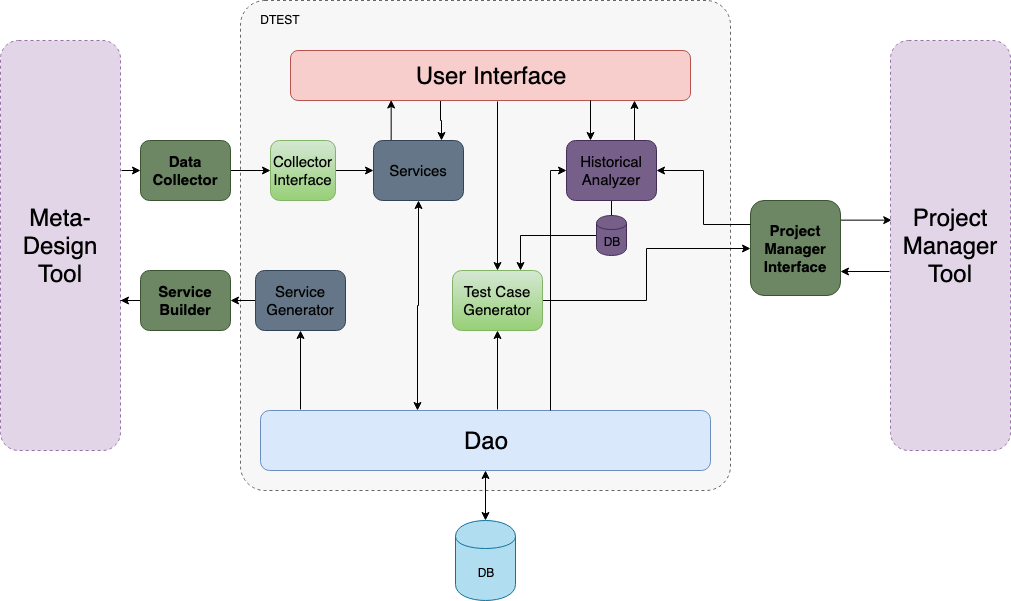
\includegraphics[width=1\textwidth]{figuras/arquitetura_sem_tester.png}
\caption{Arquitetura DTEST (Fonte: Elaborado pela Autora.)}
\label{img:architecture}
\end{figure}

O principal objetivo da ferramenta é facilitar a realização das atividades relacionadas ao processo de Transformação Digital no governo brasileiro. Dessa forma, a \itractool se baseia na utilização de ferramentas geradoras de produtos de software com base em estratégias de meta-design e EUD. Considera-se, também, que ferramentas de gerenciamento de projetos são utilizadas como forma de gerenciamento e acompanhamento das atividades do processo de transformação. Dessa forma, de acordo com o apresentado na Figura \ref{img:architecture}, a \itractool se encontra entre a ferramenta de meta-design e a ferramenta de gerenciamento de projeto utilizada pela equipe de Transformação Digital. 

O componente central da arquitetura apresentada na Figura \ref{img:architecture} agrupa os módulos da \itractool. Os módulos destacados na cor verde escuro, ``Data Collector" e ``Project Manager Interface", são módulos a parte e que devem ser definidos de acordo com o contexto em que a \itractool será utilizada. Esta estrutura de componentes objetiva a aplicabilidade da ferramenta proposta em diversos contextos, garantindo, ainda, a generalidade e replicabilidade do trabalho apresentado.

A seguir são apresentados os principais módulos envolvidos no ambiente da ferramenta \itractool.

\begin{itemize}
    \item O módulo \textit{Data Collector} é responsável pela extração de informações na ferramenta de meta-design. Esta extração pode ser realizada como a equipe desejar. No nosso contexto, a extração precisou ser feita via \textit{web crawler}, mas poderia ser feita via API ou acesso ao banco de dados, por exemplo. A partir da obtenção dos dados, estes são mapeados em entidades do tipo \textit{Service} e registrados no banco de dados para consulta dos próximos módulos. 
    
    \item O módulo \textit{Collector Interface} é responsável por definir as regras de interface para integração do módulo \textit{Data Collector}.
    
    \item O módulo \textit{Services} é responsável pelo gerenciamento do serviços extraídos. Constrói e distribui as relações entre cada entidade dos serviços, estas relações podem ser denominadas e enxergadas no código como \textit{Stages} e \textit{Fields}. Este também é responsável por registrar todas as informações de serviços no banco de dados para consulta de outros módulos. 
    
    % \del{Acho que nesse ponto ainda não foi dito o que são Stages e Fields. Acredito que, se for o caso, poderia se descrever, quando se fala da ferramenta de Meta-Design, no que consiste um serviço e como o meta-modelo faz esse mapeamento para esclarecer isso.}
    
    \item O módulo \textit{Test Case Generator} é o módulo responsável pela geração automática de casos de teste para validar determinado serviço digitizado.
    
    \item O módulo \textit{Tester Manager} é responsável pelo gerenciamento de atividades de teste. Entre os objetivos deste módulo está a Atribuição de \textit{tours} nesse caso específico para testadores com base em características de ambos testadores e tours.
    
    \item O módulo \textit{Historical Analyzer} é responsável pela análise dos dados históricos para melhoria contínua do processo de transformação. 
    
    \item O módulo \textit{Project Manager Interface} é responsável pela formatação dos dados resultantes para registro na ferramenta de gerenciamento de projeto utilizada pela equipe. Este também é responsável pela extração de informações de gerenciador de projeto para gerar informação para o módulo \textit{Historical Analyzer}.
\end{itemize}

De maneira mais detalhada, as principais funcionalidades presentes na ferramenta são apresentadas a seguir.

\subsubsection{Suporte à Validação}
\label{sec:teste}

A partir da experiência obtida com a garantia da qualidade dos serviços advindos do contexto brasileiro de Transformação Digital, foi possível definir estratégias automatizadas para maximizar a eficiência da atividade de validação. O processo de validação dos serviços se baseia na utilização do conceito de Testes Exploratórios de tal forma que possibilitou a padronização e sistematização dos casos de teste por meio dos tours. A partir desta padronização foi possível criar uma estrutura para geração automatizada de casos de teste com base nas características do SUT.

Como o contexto brasileiro de TD se baseia em estratégias de meta-design e EUD para desenvolvimento do serviços, a extração das características de cada serviço é uma atividade passível de automação. No nosso contexto, foi desenvolvido um script em Python para extração de informação de cada serviço a partir da execução de um \textbf{web crawler} na ferramenta de meta-design utilizada. A partir da obtenção de todas as informações necessárias, é possível fazer a geração automatizada de casos de teste.

A estratégia de extração de informações dos serviços digitizados segue o padrão utilizado pela ferramenta de meta-design adotada pelo governo brasileiro. Deste modo, observa-se que um \textbf{Service} possui uma ou mais \textbf{Stages} e muitos \textbf{Fields}. Entretanto, vale destacar que cada \textbf{Field} está associado a todas as \textbf{Stages} do serviço, entretanto com configurações diferentes (somente leitura, obrigatório, opcional e etc). A partir desta estrutura de relacionamento, o Algorithm \ref{test_case_generation} apresenta a lógica utilizada para geração dos casos de teste com base nas características do SUT.

    \begin{algorithm}[!htb]

	\KwIn{Service service}
	\KwResult{List tests}

	\SetKwProg{Fn}{Function}{}{}
	\Fn{generate\_test\_cases(service)}{
	   tests = []\;
	   
	   \For{service.stages as stage}{
	        tests.append(test\_cancel\_stage(stage))\;
	        
	        \For{stage.stage\_fields as stage\_field}{
	            type = verify\_type(stage\_field)\;
	            tests.append(create\_test(type, stage\_field))\;
	        
	        }
	   }
        % \If{not f\_base}{
        %     feature.save()\;
        % }
		\Return{tests}\;
	}	
	
	
	
\caption{Test Case Generation.}
\label{test_case_generation}
\end{algorithm}

A linha 3 do Algoritmo~\ref{test_case_generation} extrai todas as \textbf{Stages} de um serviço e itera sobre elas. Para cada \textbf{Stage}, um caso de teste baseado na Tour Período Chuvoso (Metáfora do Turista \cite{whittaker2009exploratory}) é gerado, validando o funcionamento correto da opção de cancelar a \textbf{Stage} atual.

Outros casos de teste genéricos para qualquer \textbf{Stage} devem ser incluídos após a linha 3 e antes da linha 5. Após a linha 5 do Algoritmo~\ref{test_case_generation}, cada relação Stage-Field é analisada para geração de casos de teste específicos com base na configuração de cada \textbf{Field} em cada \textbf{Stage}. Com esta estrutura, basta identificar casos de teste adequados a determinadas características do serviço e incluí-lo como uma nova verificação dentro do método \textit{create\_test()}. A Tabela~\ref{tab:test_types} apresenta os tipos de teste já cobertos pela \textbf{ITRACtool}.


\begin{table}[htb!]
\centering
\caption{Current types of auto-generated test cases.}
\label{tab:test_types}
\begin{tabular}{|c|c|c|}
\hline
\textbf{Field Type}                                                                   & \textbf{Test Case}                                                       & \textbf{Description}                                                                                                                                            \\ \hline
\textit{\begin{tabular}[c]{@{}c@{}}Required \\ Field\end{tabular}}                    & \begin{tabular}[c]{@{}c@{}}Test required \\ fields\end{tabular}          & \begin{tabular}[c]{@{}c@{}}Validate the exception \\ obtained with the \\ submission of the form \\ without the inclusion of \\ the required field\end{tabular} \\ \hline
\multirow{2}{*}{\textit{\begin{tabular}[c]{@{}c@{}}Normal \\ (Visible)\end{tabular}}} & \begin{tabular}[c]{@{}c@{}}Test help \\ text\end{tabular}                & \begin{tabular}[c]{@{}c@{}}Validate the help \\ text message in\\ each visible Field.\end{tabular}                                                              \\ \cline{2-3} 
                                                                                      & \begin{tabular}[c]{@{}c@{}}Test field \\ label\end{tabular}              & \begin{tabular}[c]{@{}c@{}}Verify field label \\ consistency\end{tabular}                                                                                       \\ \hline
\textit{Email}                                                                        & \begin{tabular}[c]{@{}c@{}}Test email \\ field\end{tabular}              & Validate invalid email                                                                                                                                          \\ \hline
\multirow{2}{*}{\textit{Data}}                                                        & \begin{tabular}[c]{@{}c@{}}Test Date \\ field\end{tabular}               & Validate invalid Date                                                                                                                                           \\ \cline{2-3} 
                                                                                      & \begin{tabular}[c]{@{}c@{}}Test Date \\ modal\end{tabular}               & \begin{tabular}[c]{@{}c@{}}Validate the date \\ modal format\end{tabular}                                                                                       \\ \hline
\multirow{4}{*}{\textit{Template}}                                                    & \begin{tabular}[c]{@{}c@{}}Test \\ template\end{tabular}                 & \begin{tabular}[c]{@{}c@{}}Submit an invalid format \\ or size\end{tabular}                                                                                     \\ \cline{2-3} 
                                                                                      & \begin{tabular}[c]{@{}c@{}}Test \\ template\\ specification\end{tabular} & \begin{tabular}[c]{@{}c@{}}Validate the\\ required file specification\end{tabular}                                                                              \\ \cline{2-3} 
                                                                                      & \begin{tabular}[c]{@{}c@{}}Test template \\ size\end{tabular}            & \begin{tabular}[c]{@{}c@{}}Validate the max \\ size accepted\end{tabular}                                                                                       \\ \cline{2-3} 
                                                                                      & \begin{tabular}[c]{@{}c@{}}Test template\\ modal\end{tabular}            & \begin{tabular}[c]{@{}c@{}}Validate the template \\ modal format\end{tabular}                                                                                   \\ \hline
\textit{Phone}                                                                        & \begin{tabular}[c]{@{}c@{}}Test mask\\ phone\end{tabular}                & \begin{tabular}[c]{@{}c@{}}Verify valid and invalid \\ masks for phones\end{tabular}                                                                          \\ \hline
\end{tabular}
\end{table}

Desse modo, o serviço analisado passa por uma inspeção que busca características específicas do serviço para geração de casos de teste. Como resultado da atividade de geração de casos de teste, encontra-se uma lista de casos de teste formatados de tal forma que seja possível a inclusão destes em uma ferramenta de gerenciamento de projetos, para registro e acompanhamento do caso de teste.

\subsubsection{Generation Support}
\label{sec:geracao}

% Dado que a transformação do serviços é feita a partir da utilização de ferramentas de meta-design, é possível identificar pontos de automação que possibilite maximizar a eficiência desta atividade. 
De acordo com a experiência obtida ao longo do primeiro ano de transformação digital, algumas atividades mecânicas puderam ser destacadas, como a construção do serviço, criando as \textbf{Stages} e \textbf{Fields} associados, assim como a configuração de cada \textbf{Field} em suas respectivas \textbf{Stages}. Esta atividade mecânica e repetitiva foi automatizada a partir da implementação dos módulos \textit{``Service Generator"} e \textit{``Service Builder"}, apresentados na Figura \ref{img:architecture}.

Este objetivo é alcançado a partir da definição das características do serviço desejado utilizando a \itractool, exportando essas características para a ferramenta de meta-design. A estratégia adotada para exportar o serviço foi a utilização de um \textbf{web crawler} escrito em Python, responsável por navegar pela ferramenta de meta-design e criar as \textbf{Stages} necessárias, seus respectivos \textbf{Fields} e, consequentemente, suas configurações de visualização e comportamento.

Vale ressaltar que a estratégia de geração de serviços na ferramenta de meta-design deve ser definida de acordo com as características envolvidas. Em alguns casos, algumas adaptações devem ser realizadas, de acordo com o funcionamento da ferramenta de meta-design utilizada pela equipe de transformação.

% Os conceitos utilizados para a definição da estratégia dos testes serão descritos nas seções x, y e z.

De acordo com o apresentado nesta seção, a ferramenta \itractool trabalha com diversas informações úteis para o contexto analisado nesta pesquisa. Dessa forma, a proposta de abordagem apresentada neste trabalho deverá se relacionar com a ferramenta \itractool.

\section{Testes Exploratórios}
\label{sec:testes_exploratorios}

 No contexto do ciclo de vida do desenvolvimento de software, a atividade de teste é de suma importância, visto a sua capacidade de avaliar e melhorar a qualidade do software \cite{bertolino2007software}. Existem diversas técnicas para cumprir o teste sistemático de software, seja teste caixa preta, caixa branca e caixa cinza. Dessa forma, testadores utilizam diferentes técnicas para encontrar e solucionar defeitos com o menor esforço possível \cite{maldonado2004introduccao}. 

A realização de teste por parte de testadores humanos é relevante no desenvolvimento de software do mundo real por facilitar a identificação de novos BUGs, especialmente no contexto de sistemas interativos. Testadores humanos têm vantagens sobre máquinas, visto a capacidade de conhecimento, aprendizado e adaptação a novas situações, que facilita o processo de reconhecimento eficiente de dos problemas~\cite{itkonen2015test}. 

O ato de explorar pode ser consolidado quando não se sabe ao certo qual caminho traçar para se chegar a determinado ponto, este ato é análogo ao teste de software, porque busca descobrir informações sobre a qualidade do sistema a ser testado~\cite{itkonen2015test}.

O Teste Exploratório (TE) é uma abordagem de teste manual que emerge com um potencial de adaptação para os testes a partir de um processo de aprendizagem, utilizando de uma visão mais humana e relacionada à experiência dos envolvidos. Esta abordagem de teste foi mostrada na indústria de software com seus primeiros materiais produzidos aparecendo em blogs da internet~\cite{kaner2000testing} e, em 2009, aparecendo em livros e artigos. 

O termo também aparece em \textbf{SWEBOK}~\cite{bourque2014guide}, onde é definido simultaneamente como aprendizagem, o projeto de teste 
e a execução do teste, ou seja, os testes são definidos antecipadamente em um plano de teste estabelecido, mas 
são dinamicamente projetados, executados e modificados.

Por meio do teste exploratório, é possível que o testador não dependa de um conjunto de casos de teste pré-projetados, visto que, dentro dessa abordagem de teste existem etapas de \textit{design} e execução de testes, nas quais os testadores estão constantemente aprendendo e 
adaptando suas atividades. De maneira prática, o testador aprende iterativamente sobre o produto e suas falhas, projeta e executa os testes de forma dinâmica~\cite{whittaker2009exploratory}, mas sistemática. Os tours permitem aos testadores se recordarem dos objetivos do teste e, desse modo, mesmo que os testes sejam feitos de forma manual e exploratória, a forma de exploração fica sistematizada quando testador procura atingir o objetivo do tour.

A Tabela~\ref{tab:comparativo} apresenta uma adaptação da comparação realizada por \cite{itkonen2015test}, na qual se observa a repetibilidade mecânica, orientada por documentos na execução do teste. A abordagem de testes exploratórios destaca o conhecimento, a aprendizagem e a descoberta de novas informações que proporcionam um conhecimento mais aprofundado do software. 

O teste exploratório apresenta objetivos semelhantes aos testes automatizados, entretanto, o TE não utiliza descrições formais ou metodologias detalhadas, além da não necessidade de acesso ao código-fonte, o que faz com que sua abordagem seja mais adequada ao contexto da transformação digital de serviços, parte deste trabalho. 

% Please add the following required packages to your document preamble:
% \usepackage{graphicx}
% \usepackage[table,xcdraw]{xcolor}
% If you use beamer only pass "xcolor=table" option, i.e. \documentclass[xcolor=table]{beamer}
\begin{table}[!htb]
\caption{Comparativo entre teste automatizado, teste manual (\textit{ad-hoc}) e teste exploratório. Adaptado de \cite{itkonen2015test}.}
\label{tab:comparativo}
\resizebox{\textwidth}{!}{%
\begin{tabular}{|l|l|l|l|}
\hline
\rowcolor[HTML]{333333} 
{\color[HTML]{FFFFFF} } & {\color[HTML]{FFFFFF} \textbf{Automatizado}} & {\color[HTML]{FFFFFF} \textbf{Manual (ad-hoc)}} & {\color[HTML]{FFFFFF} \textbf{Teste Exploratório}} \\ \hline
\rowcolor[HTML]{FFFFFF} 
\textbf{\begin{tabular}[c]{@{}l@{}}Filosofia \\ de Teste\end{tabular}} & Automatizado e repetitivo para oferecer feedback & \begin{tabular}[c]{@{}l@{}}Mecânico, repetitivo \\ e descrito em instruções explícitas.\end{tabular} & \begin{tabular}[c]{@{}l@{}}Conhecimento intensivo,\\ atividade criativa que requer habilidades.\end{tabular} \\
\rowcolor[HTML]{EFEFEF} 
\textbf{\begin{tabular}[c]{@{}l@{}}Design \\ de Teste\end{tabular}} & \begin{tabular}[c]{@{}l@{}}Design desafiador e caro, \\ mas de execução rápida e barata.\end{tabular} & Design separado e sequencial. & \begin{tabular}[c]{@{}l@{}}Design e execução paralelos; \\ Requer aprendizagem exploratória \\ do teste.\end{tabular} \\
\rowcolor[HTML]{FFFFFF} 
\textbf{Documentação} & \begin{tabular}[c]{@{}l@{}}Certos tipos de testes podem ser \\ roteirizados e automatizados.\end{tabular} & \begin{tabular}[c]{@{}l@{}}O teste pode ser distribuído para\\ diversos tipos de pessoas \\ com base nos testes documentados.\end{tabular} & \begin{tabular}[c]{@{}l@{}}Requer conhecimento e habilidades\\ difíceis de transferir com\\ a documentação.\end{tabular} \\
\rowcolor[HTML]{EFEFEF} 
\textbf{\begin{tabular}[c]{@{}l@{}}Conhecimentos \\ Necessários\end{tabular}} & \begin{tabular}[c]{@{}l@{}}Certos tipos de bugs podem ser \\ efetivamente detectados\\ automaticamente.\end{tabular} & \begin{tabular}[c]{@{}l@{}}Previsão de erros;\\ Resultados esperados documentados \\ para simples comparação de \\ tempo de execução.\end{tabular} & \begin{tabular}[c]{@{}l@{}}Os bugs são imprevisíveis e requerem\\ conhecimento do sistema e do domínio\\ da aplicação para detecção.\end{tabular} \\
\rowcolor[HTML]{FFFFFF} 
\textbf{Repetibilidade} & \begin{tabular}[c]{@{}l@{}}Repetibilidade e execução de testes em ciclos \\ muito curtos, mecessita de feedback rápido \\ sobre a regressão durante o desenvolvimento.\end{tabular} & \begin{tabular}[c]{@{}l@{}}Repetibilidade essencial; \\ Descrições exatas de casos de teste reduzem \\ a variação individual nos testes.\end{tabular} & \begin{tabular}[c]{@{}l@{}}Repetir os mesmos testes \\ não revela novos bugs nem\\ novas informações sobre a qualidade,\\ oferecendo pouco valor agregado.\end{tabular} \\
\rowcolor[HTML]{EFEFEF} 
\multicolumn{1}{|c|}{\cellcolor[HTML]{EFEFEF}\textbf{Automatização}} & \begin{tabular}[c]{@{}l@{}}Os testes devem ser \\ automatizados o máximo possível.\end{tabular} & \begin{tabular}[c]{@{}l@{}}Testadores humanos podem ser usados\\ para objetivos semelhantes aos da automação.\end{tabular} & \begin{tabular}[c]{@{}l@{}}A automação deve ser usada \\ para aprimorar os testes \\ e liberar recursos humanos para outros \\ tipos de atividades de teste.\end{tabular} \\ \hline
\end{tabular}%
}
\end{table}

\subsection{Metáfora do Turista}

Para sistematizar o processo de TE, \cite{whittaker2009exploratory} propôs a Metáfora do Turista, a qual consiste na analogia entre um turista em uma cidade e o teste de software. Segundo \cite{whittaker2009exploratory}, o turismo é uma mescla entre estrutura e liberdade, assim como o teste exploratório. Dessa forma, ele definiu a metáfora do turista com o objetivo de auxiliar na construção dos testes.

Na analogia apresentada, as funcionalidades dos softwares são separadas em distritos, que significam a delimitação de um espaço que se decide explorar, o que, na prática, representa as diferentes áreas do software. Além disso,  cada distrito possui um conjunto de ``tours'', que representam as diferentes maneiras de percorrer as diferentes características e funcionalidades do software. A seguir, são destacados alguns dos distritos mais utilizados pela equipe e suas respectivas ``tours'':

\subsubsection{Distrito Hoteleiro}

 É geralmente onde o turista descansa depois de um dia cheio de passeios e fica longe da agitação da viagem. Em um software, esse distrito representa os recursos secundários do aplicativo, normalmente ignorados ou deixados de lado. Em relação a este distrito, as ``tours'' utilizadas neste trabalho de pesquisa foram:

\begin{itemize}
    \item \textbf{Tour em Período Chuvoso}: Um turista pode se encontrar em um dia chuvoso e sentir vontade de tornar o passeio mais curto ou até mesmo cancelá-lo. No software, a recomendação é que o testador, ao fazer as ``tours'', use as opções que interrompem o processo do sistema. Os recursos que exigem processamento de intervalo de tempo e fornecem uma opção de cancelamento durante o preenchimento de algumas informações devem ser iniciados e cancelados, com o objetivo de verificar se as opções de cancelamento funcionam adequadamente em qualquer contexto.
    
    \item \textbf{Tour com Desinteressados}: Ao passear em uma cidade turística, alguns turistas podem parecer preguiçosos e desinteressados, não curtindo o passeio e o guia turístico pode ter que se esforçar mais para entretê-los. No contexto do software, os testadores desinteressados podem ser muito eficazes. A ``tour'' consiste em fazer o sistema funcionar fornecendo o mínimo de dados possível, forçando-o a se alinhar com valores padrão e entradas vazias.
\end{itemize}

\subsubsection{Distrito Decadente} 

Local onde costumam ocorrer alarmes constantemente. No software, essas ``tours'' têm como objetivo fornecer ações que podem causar falhas no software. As ``tours'' utilizadas nesta pesquisa foram:

\begin {itemize}
    \item \textbf {Tour Sabotador}: Todas as oportunidades para sabotar o aplicativo devem ser usadas. Nesta ``tour'', o testador deve forçar o software a iniciar alguma operação, identificar os recursos necessários para terminá-lo e remover esses recursos. Deve-se, por exemplo, solicitar que o aplicativo leia algo no disco, mas sabotar a tentativa de leitura para causar confusão, levando o sistema a falhar.
    \item \textbf {Tour Antissocial}: Em um passeio pela cidade, o turista anti-social é aquele que mostra claramente a insatisfação com o passeio e faz questão de encontrar algo para se opor a tudo o que é visto ou falado durante o passeio. Para testadores, é indispensável ter esse aspecto anti-social, com o objetivo de procurar por todos os tipos de possíveis falhas no software. A ``tour'' anti-social consiste em inserir entradas que nunca devem ser inseridas e/ou entradas que possam causar danos ao sistema.
\end {itemize}

\subsubsection{Distrito de Negócios}

É aquele em que bancos, lojas, blocos comerciais e restaurantes podem ser encontrados. Em suma, é o distrito que tem o horário comercial produtivo e as interações sociais típicas do pós-trabalho. Fazendo uma associação com software, o Distrito de Negócios é o núcleo do aplicativo, com os principais recursos que o usuário recorre no sistema. Neste distrito, as seguintes ``tours'' foram selecionadas:

\begin {itemize}
    \item \textbf {Tour Intelectual}: Os guias turísticos estão sujeitos a responder perguntas difíceis, formuladas pelos turistas com uma combinação de curiosidade e conhecimento prévio do local visitado. Para os testadores, \textit{The Intellectual Tour} consiste em uma sobrecarga do software do modo que requer mais processamento ou faz com que sua capacidade de trabalho em situações hostis seja testada.
    \item \textbf {Tour FedEx}: A FedEx é uma das maiores empresas de entrega de encomendas do mundo e faz todo o trabalho de coleta e distribuição desses pacotes para que cheguem ao seu destino final. A \textit{FedEx Tour} é baseada na noção de verificação de movimentação de dados dentro do aplicativo, testando se há algum tipo de corrupção durante esse caminho.

    \item \textbf {Tour Coletor de Lixo}: Os coletores de lixo percorrem a cidade de maneira metódica, e como resultado disso eles estão bem familiarizados com os lugares em que normalmente são alterados. O \textit{Garbage Collector Tour} consiste no testador executar o aplicativo inteiro para um propósito específico e de maneira metódica. Um exemplo seria verificar todas as mensagens de erro ou aviso fornecidas em todos os recursos do sistema.
    \item \textbf {Tour Guiado (F1)}: Guias de viagem orientam os turistas sobre os melhores lugares e atrações da cidade visitada. Trazendo-o ao contexto do software, os guias referem-se aos manuais do usuário. Também chamado de ``F1 Tour'', o Tour Guiado induz o testador a usar manuais do usuário para ajudar a explorar o software de acordo com o que eles indicam.
\end {itemize}

\subsubsection{Distrito Histórico}

É onde estão os edifícios da cidade antiga, os lugares de relevância histórica que são geralmente pontos turísticos muito populares. No software, o distrito histórico representa localizações de códigos legados, recursos mais antigos e falhas corrigidas. Apenas uma ``tour'' foi selecionada neste distrito para esta pesquisa:

\begin{itemize}
    \item \textbf {Tour à Vizinhança Ruim}: As áreas que os turistas são aconselhados a evitar existem em todas as cidades, principalmente devido a perigos e problemas estruturais da cidade. O objetivo desta ``tour'', quando nos referimos ao contexto de software, é averiguar áreas do software que costumam apresentar um alto número de defeitos. Assim, o testador se concentra mais em áreas onde a identificação de defeitos é mais provável.
\end{itemize}

%falar sobre a LECOM, fazer um overview sobre a empresa e a relação dela com o ministério, depois relacionar com a necessidade do processo de validação

% fazer um comparativo entre LECOM e Apex, só a fim de citar uma outra empresa que presta serviços pro governo.

% incluir a figura de representação do serviço digital 

%---------------- Perfil de Testadores--------------%

Como já foi levantado anteriormente, características pessoais dos testadores são atributos importantes quando se refere ao contexto de Testes Exploratórios, como mostram \cite{whittaker2009exploratory, itkonen2015test, itkonen2012role, itkonen2005exploratory}. Dessa forma, a Seção~\ref{sec:perfil_testadores} apresenta uma discussão importante sobre o perfil de testadores e seu impacto no processo de desenvolvimento, verificação e validação de software.